\section{Master project}
For my master project and thesis I will try to implement the Boids behavior on the ChIRP robots. The robots have 8 IR-LEDs and 8 IR receivers which I will use to avoid obstacles and the walls. The ChIRP robots can easily detect colored obstacles, but have some problems with black objects because they do not reflect light very well. The same goes for other robots, they do not reflect infrared light very well, due to the structure of the robots. The robot is pretty hollow at the top, where the infrared LED lights are mounted. This might impose a problem with object avoidance or the Boids' separation behavior. The quick fix for this is to physically alter the robot by adding a paper strip around robot, near the IR-LEDs which will hopefully reflect the infrared light.
The robots' PCB also have holes in it that we can use to mount various other things on top of it. These holes can be used to mount some sort of reflectors that will reflect the infrared light if the paper method does not work.
\begin{figure}[H]
\centering
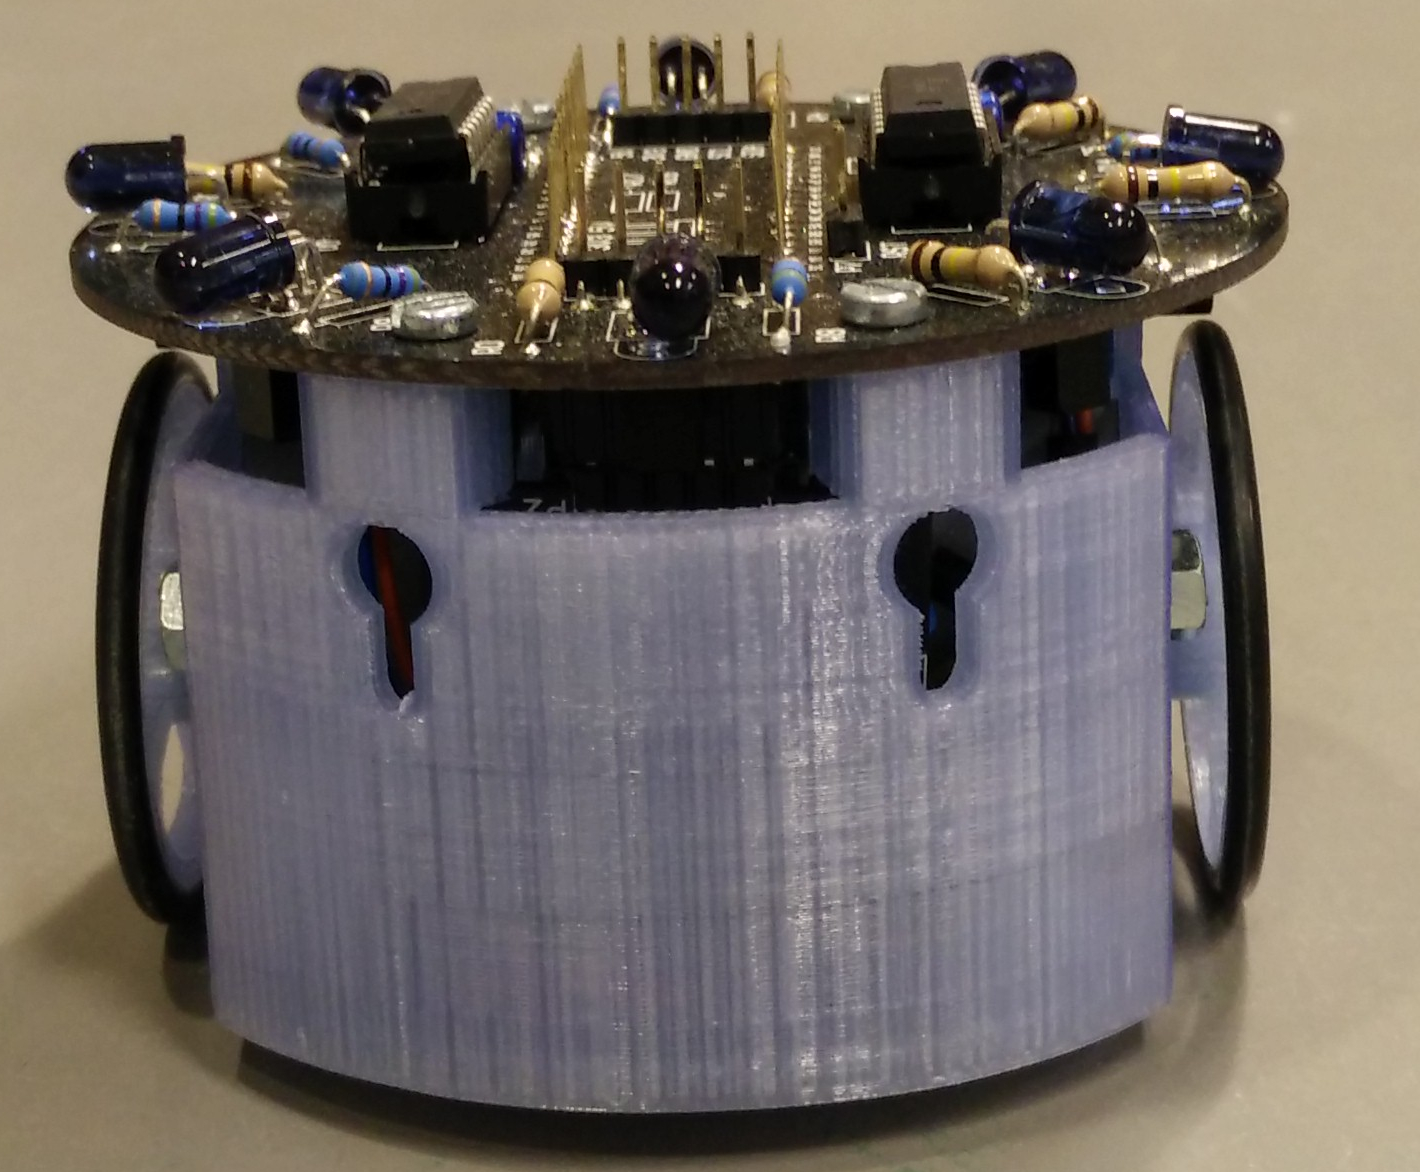
\includegraphics[width=0.8\linewidth]{images/chirpFront.jpg}
\caption[Front of ChIRP robot]{The front of the ChIRP robot, the blue IR LED on top of the robot might not reflect as good of other robots due to the structure of it}
\label{fig:chirpsFront}
\end{figure}
For now we only have 4 functional bluetooth modules that the robots can use. We have all in all 6 bluetooth modules, but we lack adapters. It is not possible to connect the bluetooth modules to the robot without these adapters. New adapters can be printed in Omega-verksted or bought from companies that prints out PCB.

Only using the IR distance sensors is not enough to find all the information needed to implement Boid behavior on the robot, namely the position of each robot and their rotation.
Each robot will therefore communicate with a computer using their bluetooth module.
This centralized computer will have an overview of the sandbox using the web camera and the tracking software found in the SVN repository and will be able to provide the robots with the information they need.

Swarming robots are not supposed to communicate with an overall centralized system, but due to the technical limitation and sensors each robot is equipped with, the alternative to communicating with a centralized system is to equip more advanced sensors on the robot, which might not be plausible.

After simple Boid behavior is implemented, I will try to implement different type of steering behaviors mentioned in the steering paper. If there is enough time, I would like to assemble some of the ChIRP robots so I can get to know the inner workings of the robots. The ChIRP robots can easily be expanded with more sensors, it would be fun to implement fleeing and pursuit behavior based on for instance the light sensors or something similar, that way we do not need to use a centralized system to tell the robots which position they need to go to or flee from.

It is also possible to create complex mazes using the projector and the camera to detect these drawings, or using the robots' light sensors to differentiate between black spots and white light on the sandbox. This can be used for path following for instance.

These robots can only move forward, backward and/or rotate. They cannot move sideways. I do not know if that will impose a problem, but real birds and particles in simulation are allowed to move sideways, for the separation behavior as shown in figure \ref{fig:boid_sep} it seems like the Boid is moving sideway. The robot might have to turn around, move in that direction and the turn back.

Before testing anything on the robots, I will need to create a simulation where I will be able to test and debug. A simulation would able to provide information that the real robots are not capable of providing, and thus it will be easier to see if the individuals are behaving like they are supposed to do. A lot of the code from the traffic simulation can be reused, but I would rewrite the Robot class, this is because the old Robot class were written with speed and rotation, instead of 2 wheel drive.

The Arduino have limited memory, only 32 KB are present on the micro board. I do not think I will exceed this limitation, but if my implementation exceed this memory cap, then I need to rewrite the code to use smaller data types. For instance a normal \textbf{int} uses 32 bits, but one might not need all of the 32 bits. It would be better to use a \textbf{byte} data type instead, which only uses 8 bits.

